%%%%%%%%%%%%%%%%%%%%%%%%%%%%%%%%%%%%%%%%%%%%%%%%%%%%%%%%%%%%%%%%%%%%%%%%
%                                                                      %
%     File: Thesis_Versat.tex                                      %
%     Tex Master: Thesis.tex                                           %
%                                                                      %
%     Author: Andre C. Marta                                           %
%     Last modified :  2 Jul 2015                                      %
%                                                                      %
%%%%%%%%%%%%%%%%%%%%%%%%%%%%%%%%%%%%%%%%%%%%%%%%%%%%%%%%%%%%%%%%%%%%%%%%

\chapter{The Versat architecture}
\label{chapter:versat}

\begin{figure}[!htb]
	\centering
	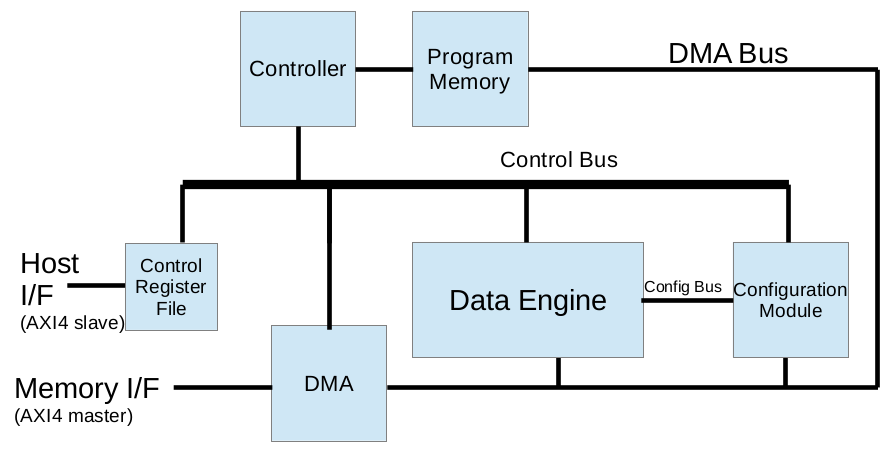
\includegraphics[width=0.8\textwidth]{Figures/top.png}
	\caption{Versat top-level entity.}
	\label{fig:top}
\end{figure}

The Versat architecture~\cite{sousa:versat, sousa:versat2016, sousa:controller,
  sousa:compiler} is shown in Figure~\ref{fig:top}, and it consists of the
following modules: Controller, Program Memory, Control Register File, DMA, Data
Engine and Configuration Module. The Controller can access the various modules
in the system via the Control Bus, and it executes programs stored in the
Program Memory (9kB = 1kB boot ROM + 8kB RAM). The user programs are loaded in
the RAM to execute algorithms which involve managing Data Engine (DE)
reconfigurations and DMA data transfers.

Versat user programs can use the DE to carry out data intensive computations. To
perform these computations, the Controller writes DE configurations to the
Configuration Module (CM) or simply restores configurations previously stored in
the CM. The Controller can also load the DE with data to be processed or save
the processed data back in the external memory using the DMA engine. The DMA
engine can also be used to initially load the Versat program or to move CGRA
configurations between the core and the external memory.

The Versat core has a host and a memory interface. Both of them use ARM’s
Advanced eXtensible Interface (AXI), a standard for busing. The host interface
(AXI slave) is used by a host system to instruct Versat to load and execute
programs. The host and the Controller communicate using the Control Register
File (CRF), an unit that is also used by Versat programs as a general purpose
(1-cycle access) register file. The memory interface (AXI master) is used to
access data from an external memory using the DMA.



%%%%%%%%%%%%%%%%%%%%%%%%%%%%%%%%%%%%%%%%%%%%%%%%%%%%%%%%%%%%%%%%%%%%%%%%
\section{Data Engine}
\label{section:data}

\begin{figure}[!htb]
	\centering
	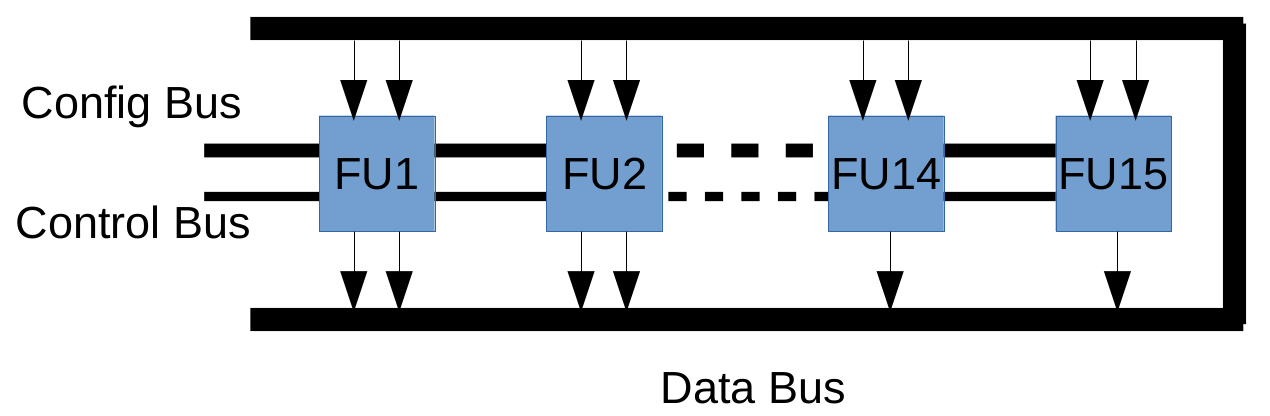
\includegraphics[width=0.8\textwidth]{Figures/de.png}
	\caption{Versat data engine.}
	\label{fig:de}
\end{figure}

The Data Engine (DE) has a flexible topology, in which the user can configure
the amount of functional units (FUs) and their respective type. In
Figure~\ref{fig:de} is shown a DE example with 15 FUs. The DE is a 32-bit
architecture with the following configurable FUs: Arithmetic and Logic Unit
(ALU), Multiplier Accumulator (MAC), Barrel Shifter (BS) and dual-port 16kB
embedded memories (MEM). The output registers of the FUs are read/write
accessible by the Controller via the Control Bus.

The FUs are interconnected by a wide bus called the Data Bus. This bus is the
concatenation of all FU outputs, with each FU contributing with a 32-bit section
to the Data Bus. An embedded memory contributes 2 sections to the Data Bus,
since it has 2 ports. These sections can be selected by each FU, according to
the configurations that they receive from the respective configuration registers
in the CM, whose outputs are concatenated in another wide bus called the Config
Bus.

The DE has a full mesh topology, meaning that each FU can select any FU output
as one of its inputs. This kind of structure may seem unnecessary but it greatly
simplifies the compiler design as it avoids expensive place and route
algorithms~\cite{sousa:versat2016}.

\begin{figure}[!htb]
	\centering
	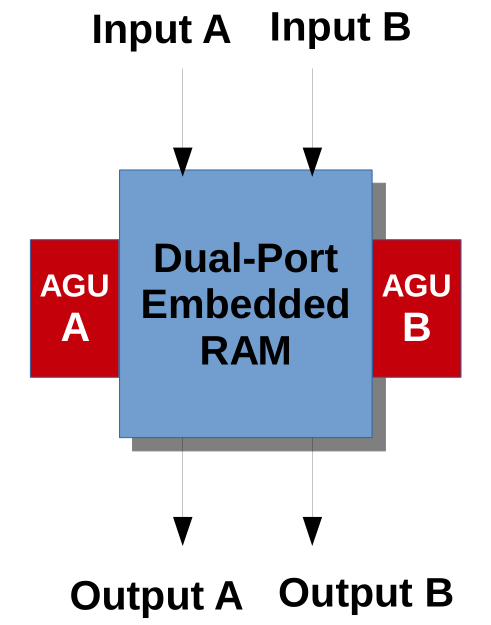
\includegraphics[width=0.23\textwidth]{Figures/memory.png}
	\caption{Versat dual-port embedded memory with AGUs.}
	\label{fig:memory}
\end{figure}

Each one of the dual-port memories used in Versat have a data input, a data
output and an address input, as shown in Figure~\ref{fig:memory}. Also, each
port has an Address Generation Unit (AGU), that can be programmed to generate
the address sequence used to access data from the memory port during the
execution of a program loop in the DE. The AGUs support two levels of nested
loops and can start execution with a programmable delay, so that circuit paths
with different latencies can be synchronized.

%%%%%%%%%%%%%%%%%%%%%%%%%%%%%%%%%%%%%%%%%%%%%%%%%%%%%%%%%%%%%%%%%%%%%%%%
\section{Configuration Module}
\label{section:configuration}

\begin{figure}[!htb]
	\centering
	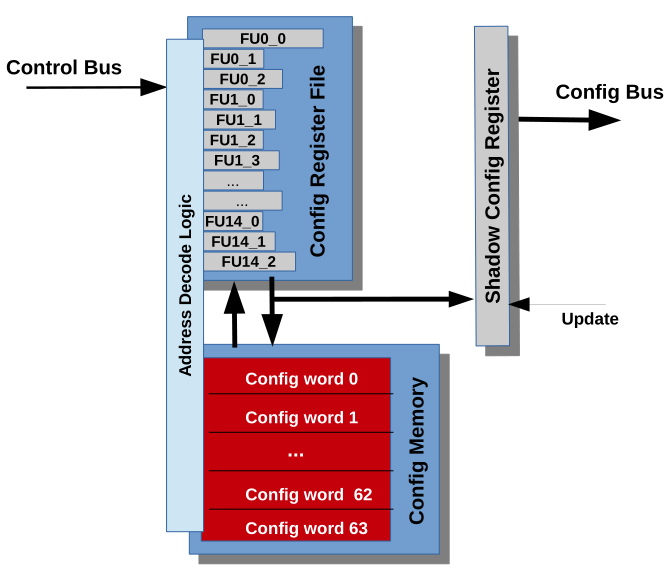
\includegraphics[width=0.6\textwidth]{Figures/configuration.png}
	\caption{Versat configuration module example.}
	\label{fig:cm}
\end{figure}

In Versat, the configuration bits are organized in configuration spaces, one for
each FU. Each configuration space comprises multiple fields, which are memory
mapped from the Controller point of view. Thus, the Controller is able to change
a single configuration field of an FU by writing to the respective address. This
implements partial reconfiguration.

A Configuration Module (CM) example is illustrated in Figure~\ref{fig:cm}, with
a reduced number of configuration spaces and fields for simplicity. It contains
a register file with a variable length (the length depends on the FUs used), a
shadow register and a memory. The shadow register holds the current
configuration of the DE, which is copied from the main configuration register
whenever the Update signal is activated. This means that the configuration
register can be changed in the main register while the DE is running.

When the CM is addressed by the Controller, the decode logic checks if the
configuration register file or the configuration memory is being addressed. The
configuration register file accepts write requests and ignores read requests. On
the other hand, the configuration memory deals with read and write requests in
the following way: a read request causes the addressed contents of the
configuration memory to be transferred into the configuration register file,
while a write request causes the contents of the configuration register file to
be stored into the addressed position of the configuration memory. This is a
mechanism for saving and loading entire configurations in a single clock cycle
because all the data transfers are internal.

%%%%%%%%%%%%%%%%%%%%%%%%%%%%%%%%%%%%%%%%%%%%%%%%%%%%%%%%%%%%%%%%%%%%%%%%
\section{Controller}
\label{section:controller}

\begin{figure}[!htb]
	\centering
	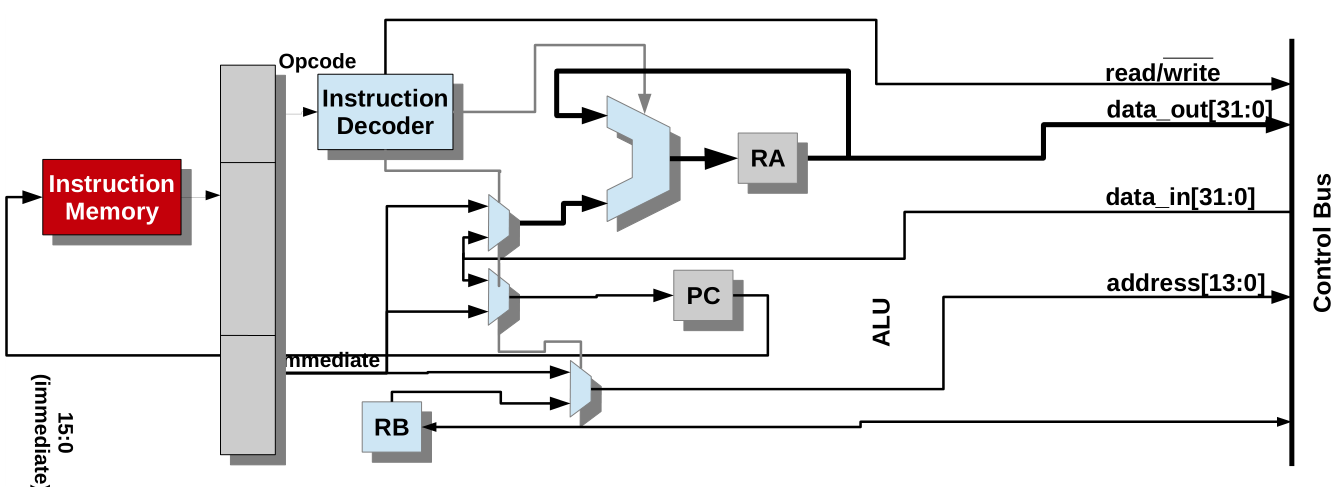
\includegraphics[width=0.8\textwidth]{Figures/controller.png}
	\caption{Versat controller.}
	\label{fig:controller}
\end{figure}

The controller used in the Versat architecture is just used for reconfiguration,
data transfer and simple algorithmic control. This controller is not meant to
replace a more general host processor, which can run complex applications while
using Versat as an accelerator.

The controller has an accumulator architecture, using a 2 stage pipeline, as
shown in Figure~\ref{fig:controller}. In this architecture 3 main registers are
used: RA, RB and PC. The RA is the accumulator, the RB is the address register,
used for indirect loads and stores, and the PC is the register that holds the
value of the program counter.

The controller is the master of a simple bus called the Control Bus, which can
be accessed using the 4 signals shown in Figure~\ref{fig:controller}. Register
RB can be accessed using the Control Bus as if it were a peripheral of the
Control Bus.

\begin{table}[!htbp]
	\centering
	\caption{Versat instruction set.}
	\label{tab:isa}
	\begin{tabular}{|c|l|}
		\hline 
		{\bf Mnemonic} & {\bf Description} \\
		\hline \hline 
		rdw & RA = (Imm)\\
		\hline
		wrw & (Imm) = RA\\
		\hline
		rdwb & RA = (RB)\\
		\hline
		wrwb & (RB) = RA\\
		\hline
		ldi & RA = Imm\\
		\hline
		ldih & RA[31:16] = Imm\\
		\hline
		beqi & RA == 0? PC = Imm: PC += 1; RA = RA-1\\
		\hline
		beq & RA == 0? PC = (Imm): PC += 1; RA = RA-1\\
		\hline
		bneqi & RA != 0? PC = Imm: PC += 1; RA = RA-1\\
		\hline
		bneq & RA != 0? PC = (Imm): PC += 1; RA = RA-1\\
		\hline
		add & RA = RA + (Imm)\\
		\hline
		addi & RA = RA + Imm\\
		\hline
		sub & RA = RA - (Imm)\\
		\hline
		shft & RA = (Imm $<$ 0)? RA=RA$<<$1: RA=RA$>>$1\\
		\hline
		and & RA = RA \& (Imm)\\
		\hline
		xor & RA = RA \^ (Imm)\\
		\hline
	\end{tabular}
\end{table}

The Versat controller Instruction Set Architecture (ISA) has 16 instructions, as
shown in Table~\ref{tab:isa}. Currently, it can only be programmed in assembly
language as it does not yet have a C compiler which is being developed by
another student working in this project.


%%%%%%%%%%%%%%%%%%%%%%%%%%%%%%%%%%%%%%%%%%%%%%%%%%%%%%%%%%%%%%%%%%%%%%%%
\section{Application Example}
\label{section:application}

During the work carried out for this report an application for an international
client using the Versat architecture was developed. It consists of an MP3
encoder, shown in Figure~\ref{fig:application}, where Versat is used to
accelerate the front end of the algorithm, denoted MP3-FE in
Figure~\ref{fig:application}).

\begin{figure}[!htb]
	\centering
	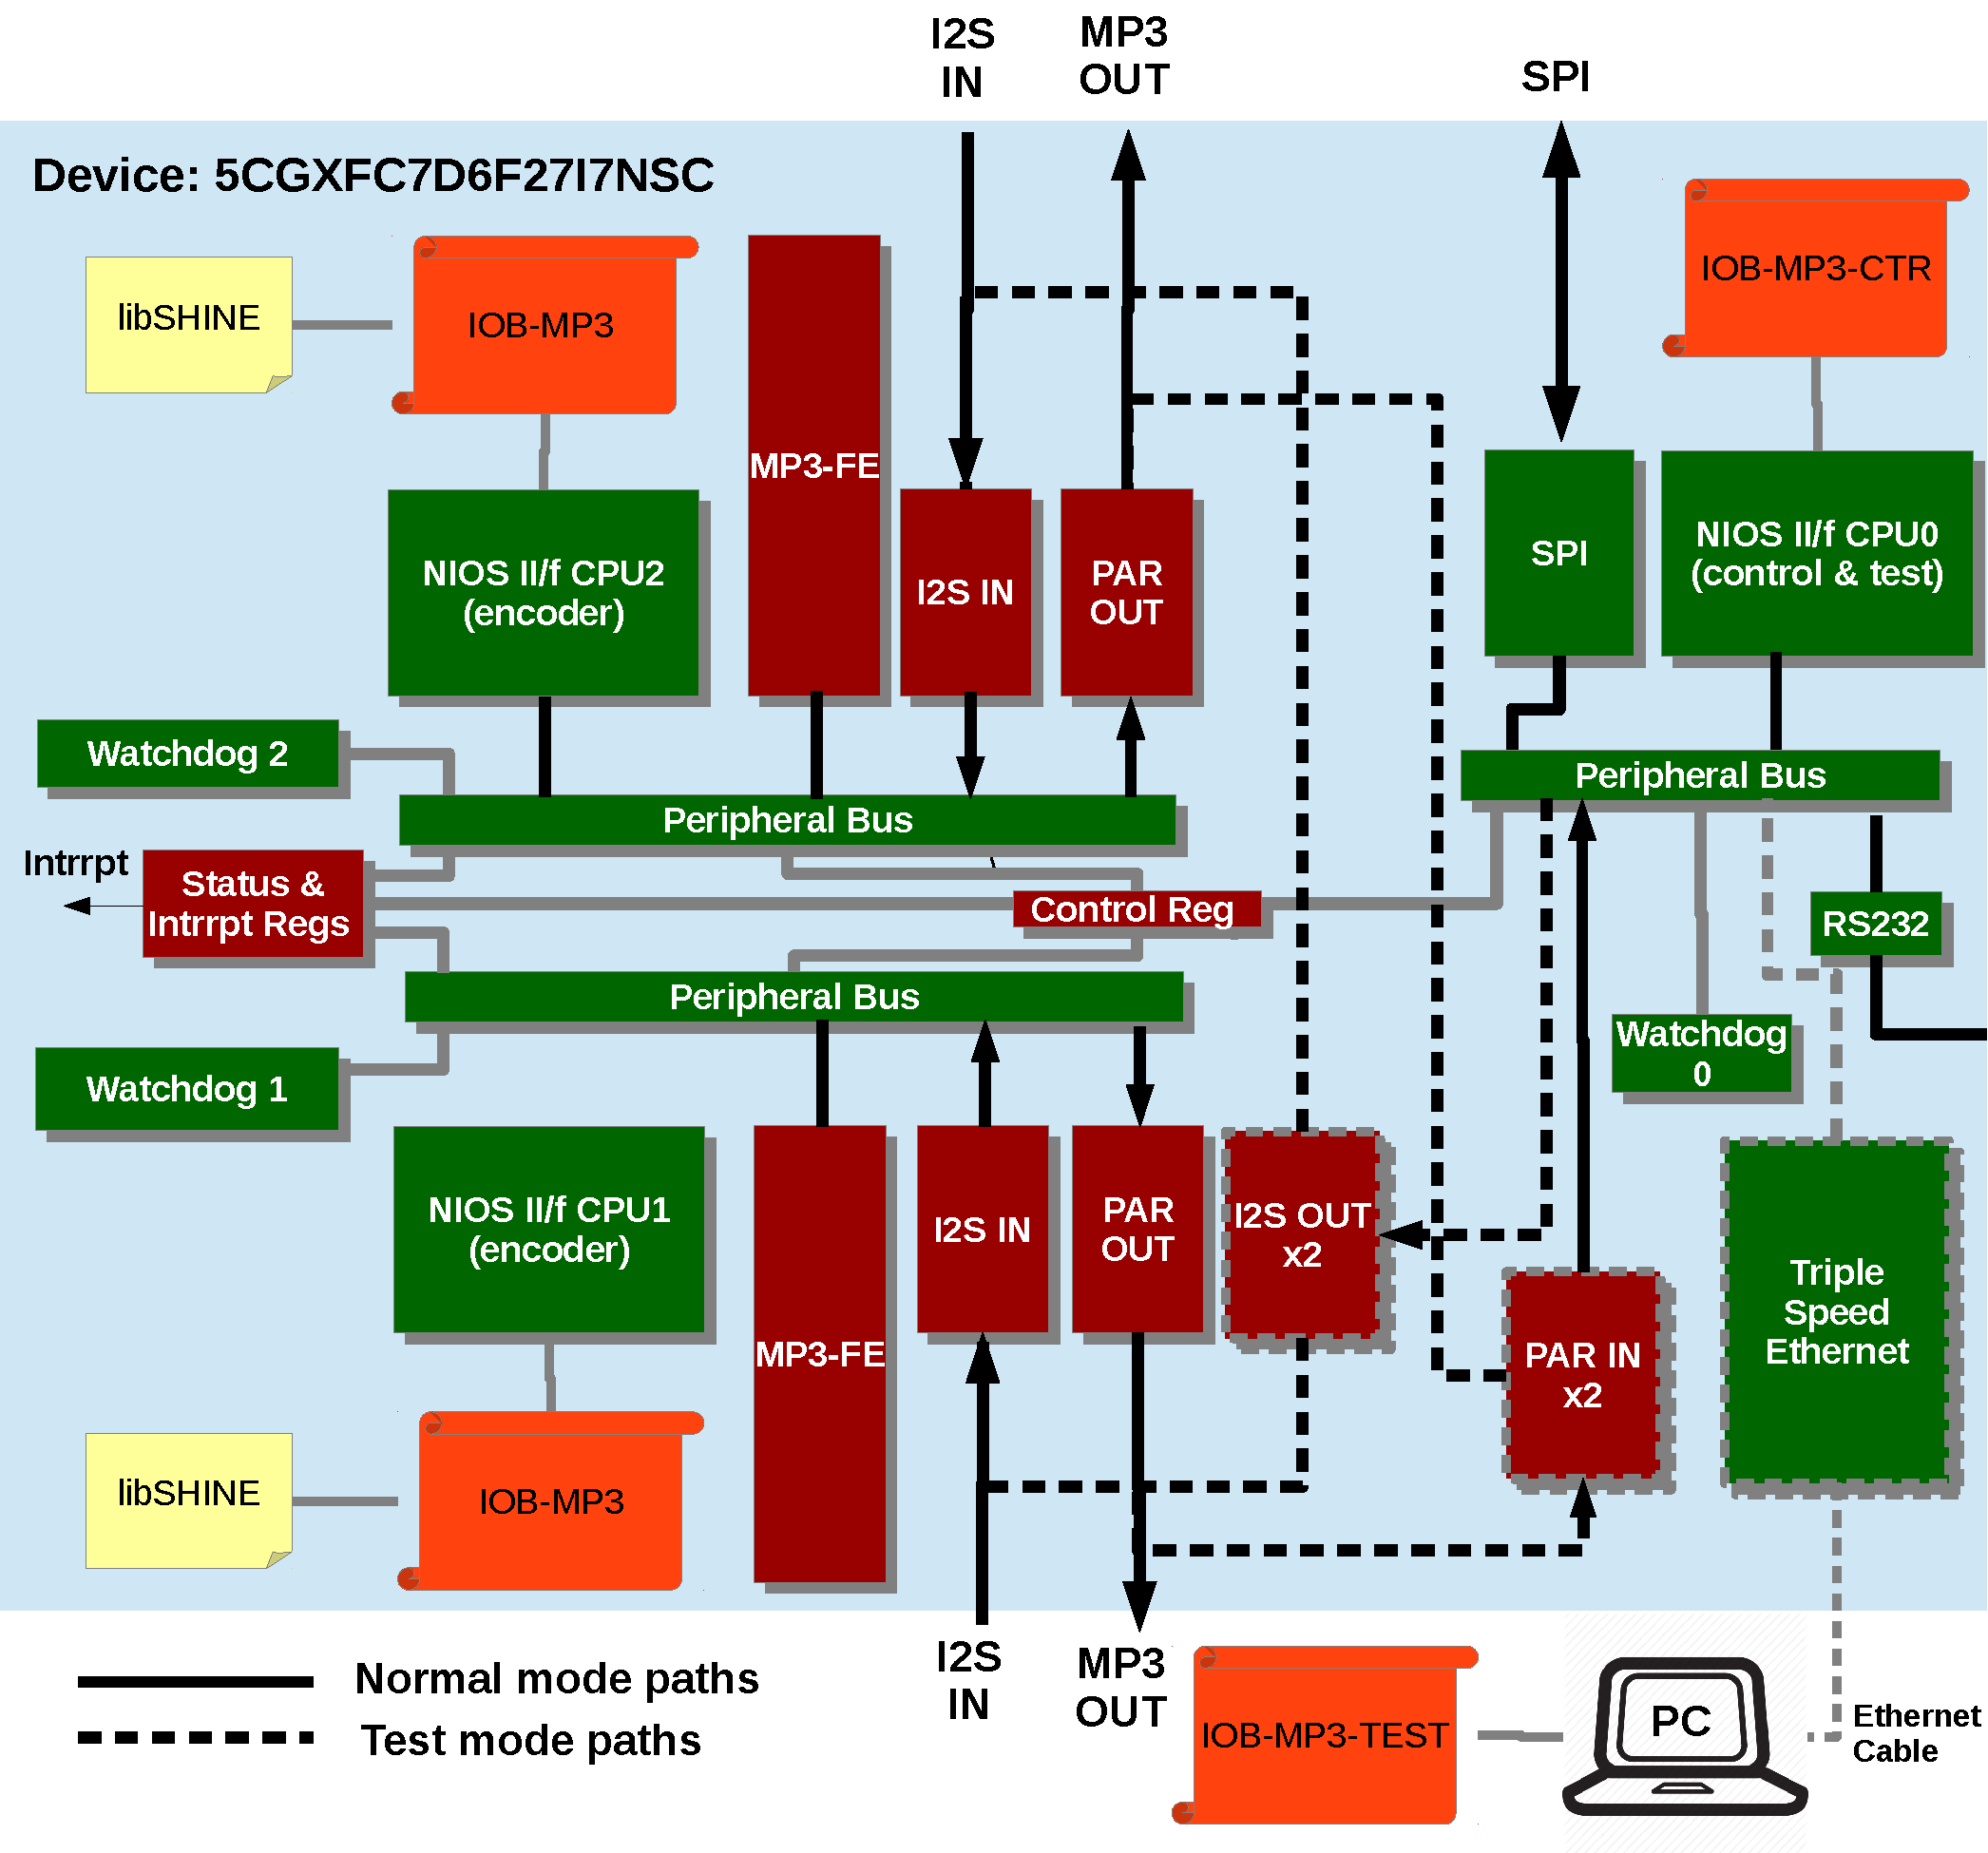
\includegraphics[width=0.85\textwidth]{Figures/bd.pdf}
	\caption{Schematic of the application where Versat was used.}
	\label{fig:application}
\end{figure}

The MP3 algorithm is based in Shine~\cite{shine:mp3}, a fast fixed-point MP3
encoding library. The front end runs sub-band filtering of the audio signal and
applies the Modified Discrete Cosine Transform to the result. These functions
are the most computationally expensive functions in the MP3 algorithm and
normally require DSP extensions to the ISA of the processor used. In the
approach taken, a more modest processor was used (Intel's NIOS2) which used
Versat as a peripheral acceleration core.

To run this algorithm the Versat architecture was configured with 4 dual-port
memories and 3 FUs: a Multiply Accumulate Unit (MAC), a simple Arithmetic and
Logic Unit (ALU) and a Barrel Shifter Unit (BS). The MP3 front-end was written
in the Versat Assembly language, since Versat compiler does not support yet the
use of a higher level programming language (like C or C++).

The FE was intensively simulated before synthesis and implementation in the
FPGA. Initially, the simulations were performed using Icarus
Verilog~\cite{icarus:verilog}, an open-source Verilog simulator. However, as the
complexity of the core increased, the simulation times also increased
dramatically, since Icarus Verilog is a fairly slow simulator, as will be seen
in section~\ref{section:performance}, where the performance of the different HDL
simulators is analysed.

As a result, at a certain point in the project, the simulator was changed to
Cadence NCSim~\cite{cadence:ncsim} to speed up the simulations. Despite NCsim
being considerably faster than Icarus Verilog, the simulations still took a
considerable amount of time. This reinforces the need for a faster simulation
environment for the Versat architecture.
